% https://topanswers.xyz/tex?q=1836#a2067
\documentclass{beamer}
\usepackage{tikz}

\begin{document}
	
\begin{frame}
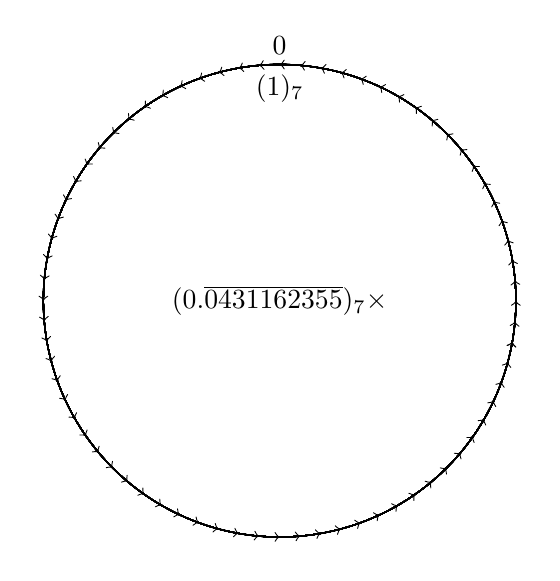
\begin{tikzpicture}
\path (0,0) circle [radius=3.2];
\foreach \x in {0,5,...,360}{
  \draw<+>[overlay,->] (\x:3) arc (\x:350+\x:3);
}
\node at (0,0) {$(0.\overline{0431162355})_{7} \times$};
\node [anchor= 90] at (90:3) {$(1)_7$};
\node [anchor=-90] at (90:3){0};
\end{tikzpicture}
\end{frame}	
	
\end{document}